\documentclass{article}
\usepackage{blindtext}
\usepackage{titlesec}
%\usepackage[utf8]{inputenc}
\usepackage{listings}
\usepackage{amsmath}
\usepackage{graphics}
\usepackage{amssymb} 
\usepackage{amsthm}
\usepackage{graphicx}
\usepackage{hyperref}
\usepackage{biblatex}
\usepackage{xcolor}
\usepackage{fancyhdr}
\usepackage{float}

\hypersetup{
    colorlinks=true,
    breaklinks=true,
    urlcolor=blue,           % set the color of hyperlinks to blue
    linkcolor=black,           % set the color of internal links (index, figures, tables, equations, etc.) to red
    citecolor=green,         % set the color of links to bibliographic references to green
}


\begin{document}
\begin{titlepage}
\begin{figure} 

\includegraphics[width=0.4\textwidth]{images/cnrslogo.jpeg}

\includegraphics[width=0.4\textwidth]{images/inria.png}
    \centering
\end{figure}

\centering
\title{}\author{}\date{}
\centering
\vspace{3cm}
{\bfseries\LARGE CNRS Alsace delegation - INRIA \par}
\vspace{4cm}
{\bfseries\LARGE Training augmented interpolation \par}
\vspace{1cm}
{\Large FONSECA HINCAPIÉ Diana Sol Angel\par}
\vspace{1cm}
{\Large STAGE M1 CSMI \par}
\vspace{3cm}
{\Large Supervisors: \par}
\vspace{0.5cm}
{\Large M.FRANCK Emmanuel\par}
\vspace{0.5cm}
{\Large M.NAVORET Laurent\par}
\end{titlepage}


%Table of contents
\maketitle
\tableofcontents 
\newpage






\section{Introduction}
%Say something about like the importance of the transport equation and the need to solve it numerically and the use of neural networks 
The focus of my internship was on solving simple transport equations using deep learning techniques, specifically Physics-Informed Neural Networks (PINNs). I will discuss the importance of solving transport equations numerically and the role of neural networks in this process.

I will provide a theoretical framework for understanding the Semi-Lagrangian scheme with augmented interpolation and PINNs, in the implementation section, I will describe the code developed for the PINNs approach, including the optimization process. I will also provide code snippets and explanations of the most important parts of the code.

In the results section I will present the outcomes of the PINNs implementation, including the results of unsupervised and supervised learning.

Finally, I will draw conclusions based on the findings and discuss the implications of the work.

\newpage

\section{General context}

The intership project was supervised by Emmanuel Franck and Laurent Navoret researchers on the development of numerical methods to solve partial differential equations for the simulation of physical phenomena from the French National Institute for Research in Computer Science and Control (INRIA) which is a leading research institution focused on computer science, applied mathematics, and control theory. 
The work is done in collaboration with the INRIA and the French National Centre for Scientific Research (CNRS)
%DONNER PLUS DE CONTEXTE

\section{Objectives}

We are interested in solving simple transport equations, the aim is to find a way to increase the accuracy of the method using deep learning techniques while keeping the guarantees of convergence.
For this we consider a simple case of deep interpolation where we approximate the solution of our transport equation by training a physics informed neural network.
We used a machine learning framework like PyTorch to implement PINNs. 

\section{Theoretical Framework}

\subsection{Lagrange interpolation}

We choose $n$ points inside $\left(x_1, \ldots, x_m\right)$.
The Lagrange interpolation operator is defined as it follows:
$$
\mathcal{I}_h^m(f)(x)=\sum_{i=1}^m f\left(x_i\right) P_i(x)
$$
with $P_i\left(x_j\right)=\delta_{i j}$


\subsection{Semi-Lagrangian Scheme}


The semi-Lagrangian scheme is a numerical method to solve transport equations. It is based on the following idea for the 1D case:


First to allow long time-steps, we construct the numerical domain of dependence to contain the physical domain of dependence.


We have an uniform grid for space $\left[x_1, \ldots x_N\right]$ and one  for the time $\left[t_1, . . t_n\right]$ with $\Delta t=t_{i+1}-t_i$ and $\Delta x=x_{i+1}-x_i$.\\
The numerical solution can be computed using the following scheme
$$
u\left(t_{n+1}, x_{jd}\right)=u\left(t_n, x_j-a \Delta t\right)= u (t_{n+1},x_{*})
$$


\begin{figure}[!h]
\centering
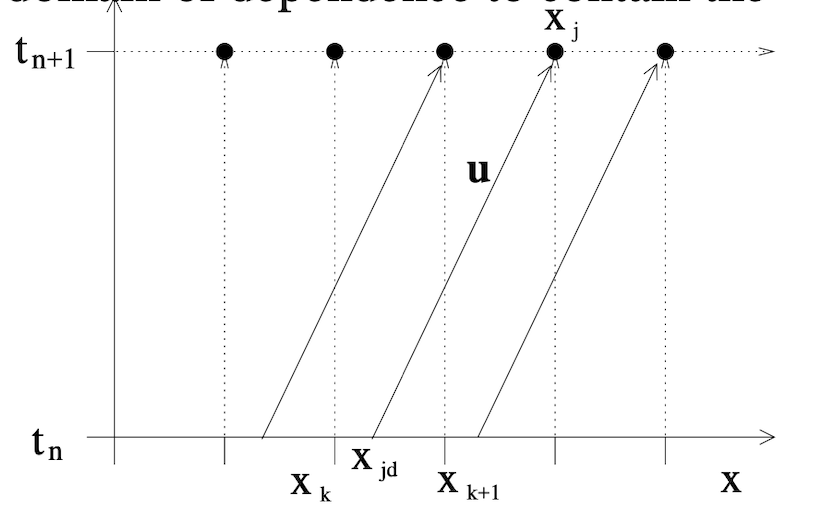
\includegraphics[width=0.4\textwidth]{images/11.png}
\caption{Semi-Lagrangian Scheme}


\end{figure}


With  $x_{*}= x_{j}-a \Delta t$ but we can clearly see that our  $x_{*}$ is not a point of our mesh and consequently we cannot know $u\left(t_n, x_i-a \Delta t\right)$. Is in at this point that we make use of the following scheme.
$$
u\left(t_{n+1}, x_i\right)=\mathcal{I}_h^m\left(u\left(t_n, x\right)\right)\left(x_i-a \Delta t\right)
$$


Where we interpolate u at time $n+1$ from the n-closest points at time $n$ and onto $x_{*}$, using our Lagrange interpolation operator described before $\mathcal{I}_h^m$ uses the $n$ points around $\left(x_i-a \Delta t\right)$.\\


\begin{figure}[!h]
\centering
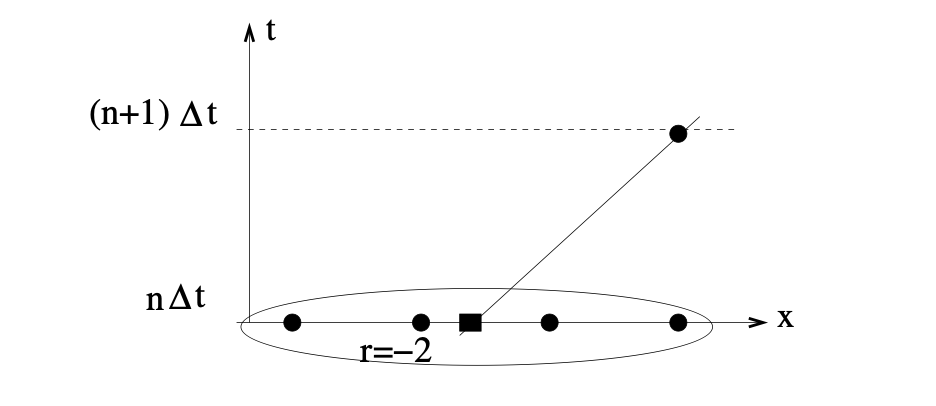
\includegraphics[width=0.5\textwidth]{images/12.png}
\caption{N-closest points for interpolation}
\end{figure}


\begin{figure}[!h]
\centering
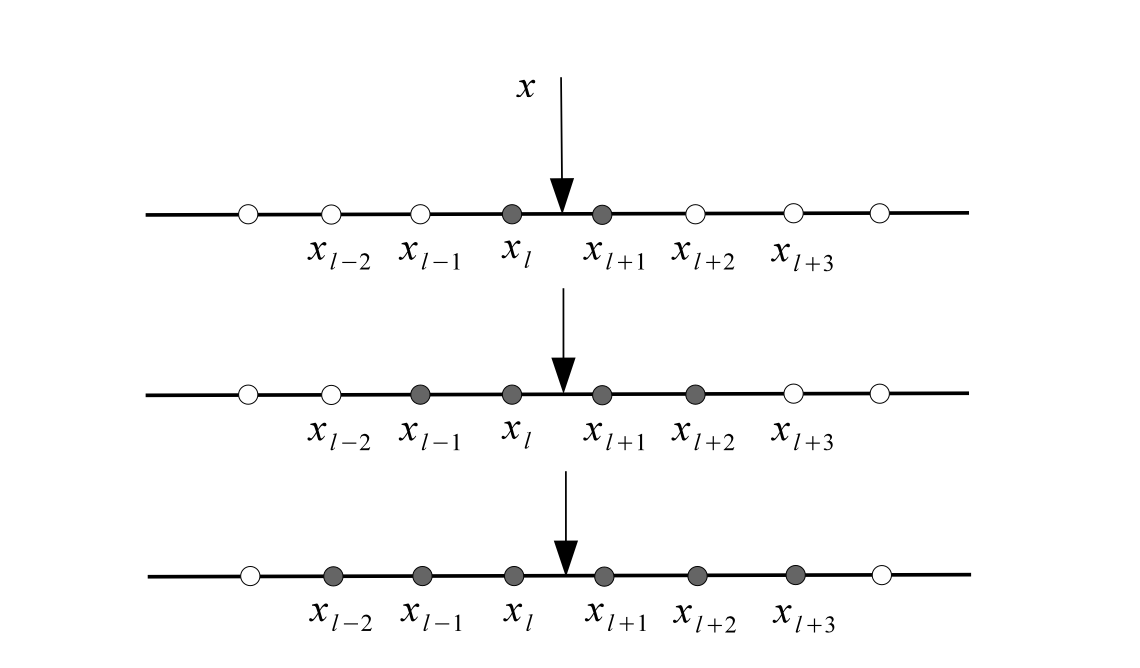
\includegraphics[width=0.5\textwidth]{images/13.png}
\caption{Different interpolation options}
\end{figure}

Then  $u\left(t_{n+1}, x_i\right)$ is the s the numerical solution computed at $\left(t_{n+1}, x_i\right)$. it is an implicit equation that needs to be solved in an iterative way.
Such a procedure is called Semi-Lagrangian because the discrete solution is given on a Eulerian fixed mesh, but on the other hand the scheme relies on the construction of $u\left(t_n, x_j-a \Delta t\right)$ which is used to approximate  $u\left(t_{n+1}, x_j\right)$.


\subsection{Augmented Interpolation}

\subsubsection{Deep Lagrange Interpolation}
The deep Lagrange interpolation operator is definded as follows:
\begin{equation*}
    \mathcal{I}_d^m(f)=\sum_{i=1}^n \frac{f\left(x_i\right)}{u_{\theta_i}\left(x_i\right)} P_i(x) u_{\theta_i}(x)
\end{equation*}

with $P_i\left(x_j\right)=\delta_{i j}$

Using this choice, we obtain that $\mathcal{I}_d(f)\left(x_i\right)=f\left(x_i\right)$ as the classical Lagrange interpolation operator. 

\subsubsection{Deep Lagrange interpolation with PINNs}

We will consider a specific case of the deep interpolation:
$$
\mathcal{I}_d^m(f)=\sum_{i=1}^n \frac{f\left(x_i\right)}{u_\theta\left(x_i\right)} P_i(x) u_\theta(x)=\mathcal{I}^m\left(\frac{f}{u_\theta}\right) u_\theta(x)
$$
This interpolation will be better than the classical one if $\frac{f}{u_\theta} \approx=1$ since we have the following error on the interpolation:
$$
\left\|f-\mathcal{I}_d^m(f)\right\|_{H^m} \leq C h^{m+1}\left\|\left(\frac{f}{u_\theta}\right)^{\prime \prime}\right\|_{L^2}\|f\|_{H^m}
$$

Now we the question is how choose $u_\theta(x)$. We propose to use a neural network which will approximate the $u_\theta(x)$ function. 

$$
u_\theta\left(x ; t, \mu, a(x), a^{\prime}(x)\right)
$$

We will train these neural networks with a \textbf{Physics Informed Neural Network} strategy and we will use the previous interpolation to approximate the solution of the PDE.

\subsection{Supervised and unsupervised learning}

\subsubsection{Supervised learning}

Supervised learning is a subcategory of machine learning and artificial intelligence. 
It is defined by its use of labeled datasets to train algorithms that to classify data or predict outcomes accurately. As input data is fed into the model, 
it adjusts its weights until the model has been fitted appropriately, which occurs as part of the cross validation process. Supervised learning uses a training set to teach models to yield the desired output. This training dataset includes inputs and correct outputs, which allow the model to learn over time. The algorithm measures its accuracy through the loss function, 
adjusting until the error has been sufficiently minimized. 

\subsubsection{Unsupervised learning}
Unsupervised learning uses machine learning algorithms to analyze and cluster unlabeled datasets. These algorithms discover hidden patterns or data groupings without the need for human intervention. Its ability to discover similarities and differences in information make it the ideal solution for exploratory data analysis, cross-selling strategies, customer segmentation, and image recognition.


In our context we will be interested in both supervised and unsupervised learning. We will use supervised learning to train the neural networks without knowing the solution and unsupervised learning to learn from the data calculated based on the exact solution of the PDE.

\subsection{Neural Networks}

Neural networks process training data by mimicking the interconnectivity of the human brain through layers of nodes, each node is made up of inputs, weights, a bias (or threshold), and an output. If that output value exceeds a given threshold, it “fires” or activates the node, passing data to the next layer in the network. Neural networks learn this mapping function through supervised learning,
adjusting based on the loss function through the process of gradient descent. When the cost function is at or near zero, we can be confident in the model’s accuracy to yield the correct answer.

They are basically functions that map an input $X$ to an output $Y$ by performing successive linear and nonlinear transformations. The linear transformations are represented by a set of weights $W$ and biases $b$ and the nonlinear transformations are represented by activation functions $\sigma$. The output of a neural network is given by:

$$\overline{u_\theta}(X)=W_n\sigma_{n-1}(W_{n-1}\sigma_{n-2}(...(W_2(W_1X+b_1)+b_2)+..)+b_{n-1})+b_n$$

\begin{figure}[H]
    \centering
    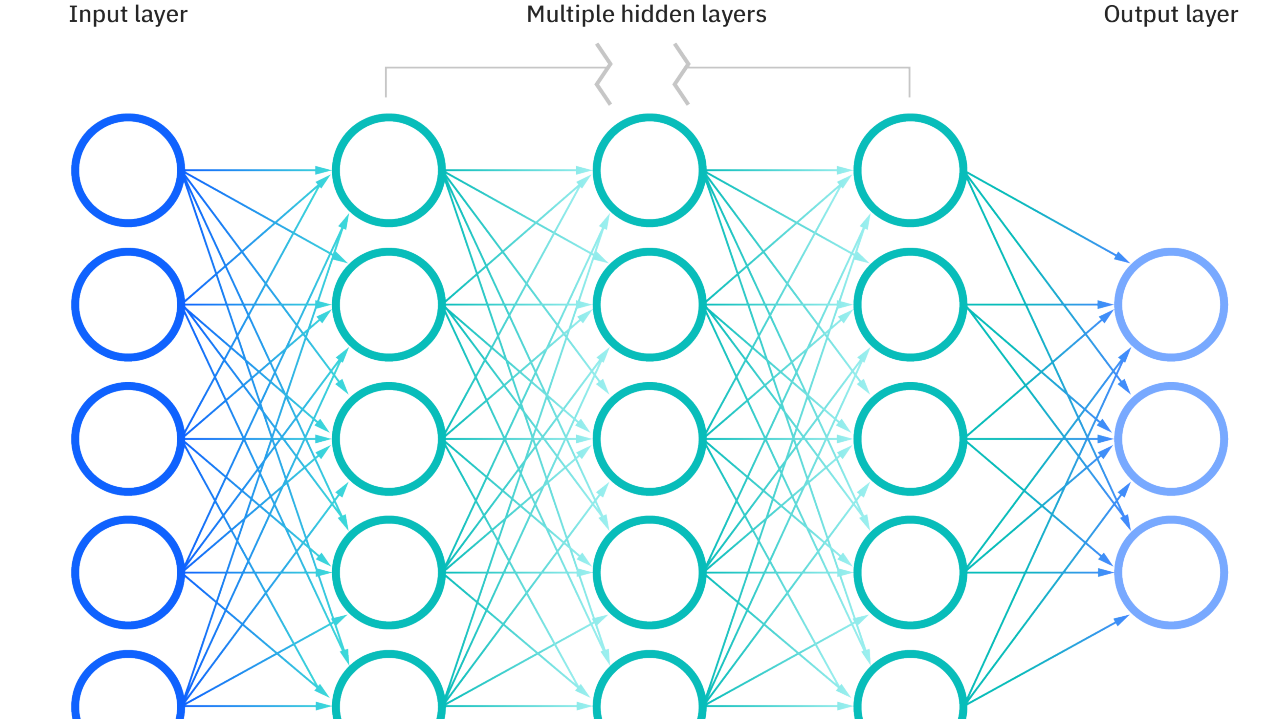
\includegraphics[width=0.5\textwidth]{images/neural_network.png}
    \caption{Neural Network Architecture}
\end{figure}
%Ajouter plus après
\subsubsection{Feed-forward Neural Network (FFNN)}

A Feed Forward Neural Network is an artificial neural network in which the connections between nodes does not form a cycle. 
The opposite of a feed forward neural network is a recurrent neural network, in which certain pathways are cycled. 
The feed forward model is the simplest form of neural network as information is only processed in one direction. While the data may pass through multiple hidden nodes, 
it always moves in one direction and never backwards. In this projetc we will be implementing a FFNN for the PINN.

\subsubsection{Multi Layer Perceptron (MLP)}

A Multilayer Perceptron has input and output layers, and one or more hidden layers with many neurons stacked together. And while in the Perceptron the neuron must have an activation function that imposes a threshold, like ReLU or sigmoid, neurons in a Multilayer Perceptron can use any arbitrary activation function.
Multilayer Perceptron falls under the category of feedforward algorithms, because inputs are combined with the initial weights in a weighted sum and subjected to the activation function, just like in the Perceptron. But the difference is that each linear combination is propagated to the next layer.
Each layer is feeding the next one with the result of their computation, their internal representation of the data. This goes all the way through the hidden layers to the output layer.
But it has more to it.
If the algorithm only computed the weighted sums in each neuron, propagated results to the output layer, and stopped there, it wouldn’t be able to learn the weights that minimize the cost function. If the algorithm only computed one iteration, there would be no actual learning.

\begin{figure}[H]
    \centering
    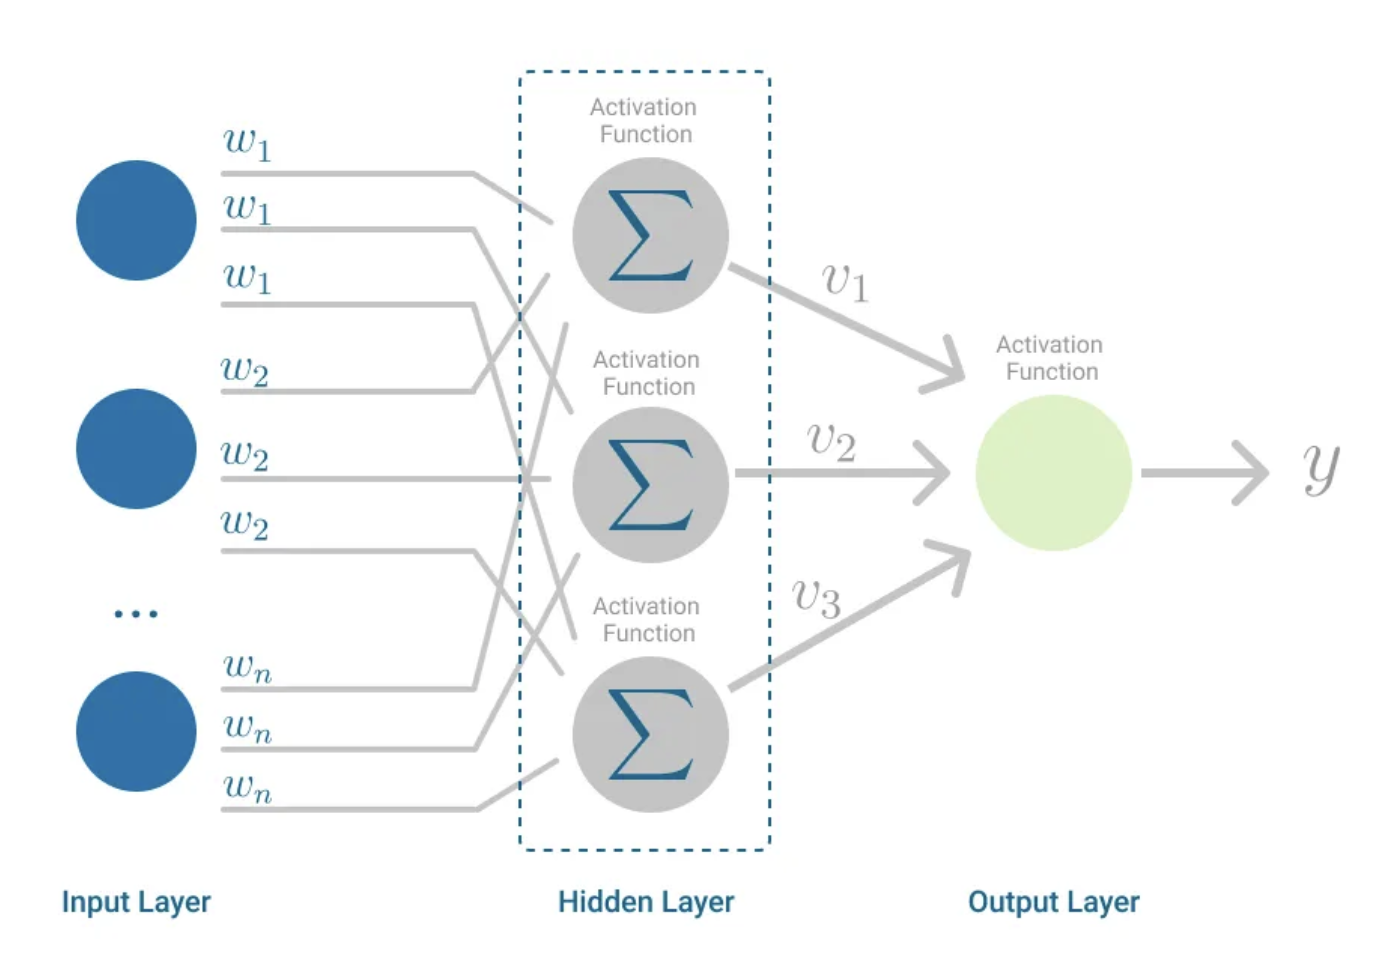
\includegraphics[width=0.5\textwidth]{images/MLP.png}
    \caption{Multi Layer Perceptron}
\end{figure}

\subsubsection{Backpropagation}

Backpropagation is a learning mechanism that allows the Multilayer Perceptron to iteratively adjust the weights in the network, with the goal of minimizing the cost function.
There is one hard requirement for backpropagation to work properly. The function that combines inputs and weights in a neuron, for instance the weighted sum, and the threshold function, for instance ReLU, must be differentiable. These functions must have a bounded derivative, because Gradient Descent is typically the optimization function used in MultiLayer Perceptron.
In each iteration, after the weighted sums are forwarded through all layers, the gradient of the Mean Squared Error is computed across all input and output pairs. Then, to propagate it back, the weights of the first hidden layer are updated with the value of the gradient. That’s how the weights are propagated back to the starting point of the neural network

Then we get the following infographic that shows the whole process of a Multilayer Perceptron with feedforward and backpropagation:

\begin{figure}[H]
    \centering
    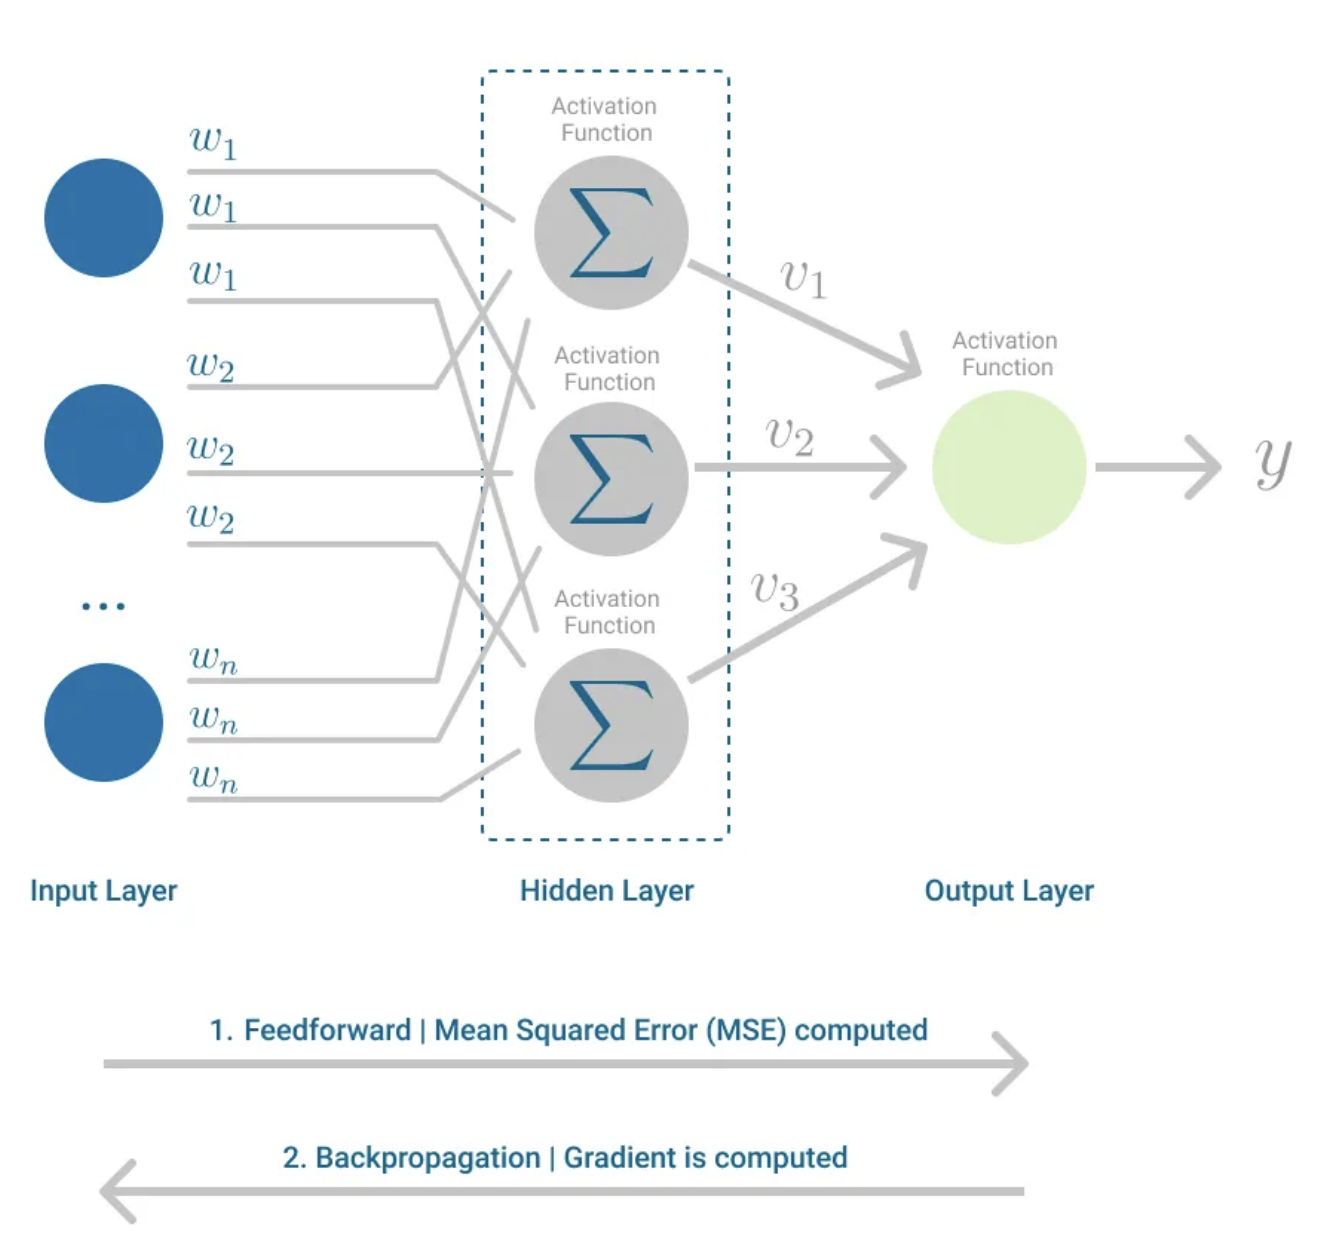
\includegraphics[width=0.5\textwidth]{images/MLP2.png}
    \caption{Multi Layer Perceptron and Backpropagation}
\end{figure}

\subsubsection{Activation functions}

The activation function that we choose for out neural network has an impact or its training. There are many commonly used activation functions like Sigmoid, Tanh, ReLU, we usually use the infinitely differentiable hyperbolic tangent activation function $tanh(x)$ that is perfect for 
PINN. The regularity of PINNs can be ensured by using smooth activation functions like as the sigmoid and hyperbolic tangent, allowing estimations of PINN generalization error to hold true

\subsubsection{Universal Approximation Theorem}

The representational ability of neural networks is well established. According to the universal approximation theorem:
The universal approximation theorem states that any continuous function  $$f : [0, 1]^{n} \rightarrow [0, 1]$$  can be approximated arbitrarily well by a neural network with at least 1 hidden layer with a finite number of weights.
Even if neural networks can express very complex functions compactly, determining the precise parameters (weights and biases) required to solve a specific PDE can be difficult.


\subsection{Physics Informed Neural Networks}

Physics-informed neural networks (PINNs) are a type of universal function approximators that can embed the knowledge of any physical laws that govern a given data-set in the learning process, and can be described by partial differential equations (PDEs).

They approximate PDE solutions by training a neural network to minimize a loss function; it includes terms reflecting the initial and boundary conditions along the space-time domain’s boundary and the PDE residual at selected points in the domain (called collocation point). 
they are deep-learning networks that, given an input point in the integration domain, produce an estimated solution in that point of a differential equation after training. Incorporating a residual network that encodes the governing physics equations is a significant novelty with PINNs. 

The basic concept behind PINN training is that it can be thought of as an unsupervised strategy that does not require labelled data, such as results from prior simulations or experiments.
It works by integrating the mathematical model into the network and reinforcing the loss function with a residual term from the governing equation, which acts as a penalizing term to restrict the space of acceptable solutions.

PINN can be viewed as an unsupervised learning approach when they are trained solely using physical equations and boundary conditions for forward problems; however, for inverse problems or when some physical properties are derived from data that may be noisy, PINNs can be considered supervised learning when they are trained using the data from the calculation of the exact solution of the PDE.
\begin{figure}[H]
    \centering
    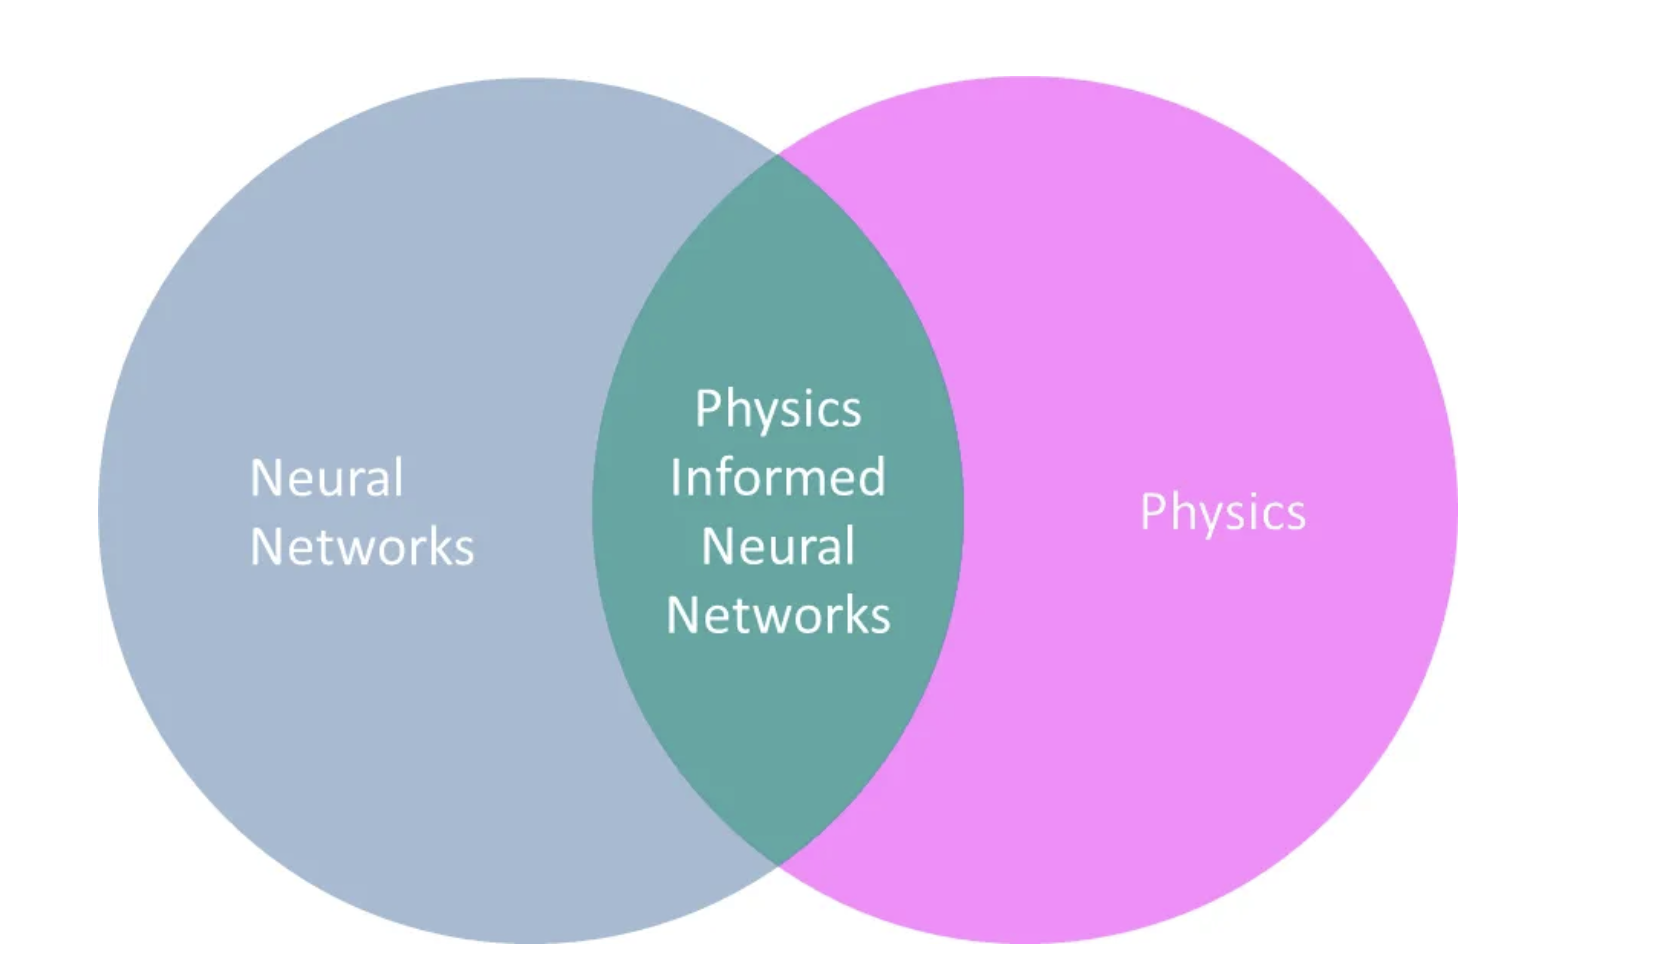
\includegraphics[width=0.5\textwidth]{images/pinns}
    \caption{PINNs}
\end{figure}

% PINNs​ = ​Data​ + ​Neural​Networks​ + ​Physical​Laws

\subsubsection{Architecture of PINNs}

% PINNs are composed of three components: a neural network, a physics-informed network, and a feedback mechanism. The first block is a NN, u_theta, that accepts vector variables and outputs the field value u. The second block can be thought of as PINN's functional component, as it computes the derivative to determine the losses of equation terms, as well as the terms of the initial and boundary conditions of the PDE. Generally, the first two blocks are linked using algorithmic differentiation, which is used to inject physical equations into the NN during the training phase. Thus, the feedback mechanism minimizes the loss according to some learning rate, in order to fix the NN parameters vector theta of the NN u_theta. In the following, it will be clear from the context to what network we are referring to, whether the NN or the functional network that derives the physical information.

%ajouter une fois que j'ai la bonne architecture qu'on va utiliser pour le PINN
% \begin{figure}[H]
%     \centering
%     \includegraphics[width=0.5\textwidth]{images/archpinns.png}
%     \caption{PINNs}
% \end{figure}



% \subsubsection{Training PINNs} AUN NO SEGURO  SI poner esta parte 


\subsubsection{Soft and Hard Constraints}

Boundary constraints can be viewed in two ways: as penalty term (soft BC enforcement) or as part of the network design (hard BC enforcement). In many existing PINN frameworks, a soft approach is taken to enforce the BCs by introducing additional loss components defined on the border's collocation points.

However, this technique has two drawbacks: it does not guarantee accurate satisfaction of the BCs, and there is no theory to guide the determination of the weights assigned to the BC loss.

There is also the hard approach to address the boundary conditions by incorporating a specific component in the neural network solely dedicated to meeting the conditions. Thus, the initial boundary conditions are considered as part of the labeled data constraint.

% Compared to the commonly used residual-based loss functions, the variational energy-based loss function is simpler to minimize and yields better results. The loss function can be constructed using collocation points, weighted residuals derived from the Galerkin-Method, or an energy-based approach. 

% There are different approaches for constructing the loss function there is the one including data-driven (without a physics model), PDE-based. 


\subsubsection{The Loss Function}

Using the PINN approach we determine the parameters $\theta$ of the NN, $u_\theta$, by minimizing the loss function:

$$
\theta = argmin_\theta L(\theta)
$$
Where the loss function is defined as:
$$
L(\theta) = L_{data}(\theta) + L_{physics}(\theta) + L_{SBC}(\theta) + L_{TBC}(\theta)+ L_{IC}(\theta)
$$

\subsubsection*{Data Loss}

The data loss is the mean squared error between the NN output and the validation of known data points, it employs the data points to train the NN, so it's a supervised learning approach.
The NN parameters are chosen by minimizing the difference between the observed outputs and the model’s predictions for the observed inputs.
$$
L_{data}(\theta) = \sum_{i=1}^{N} |u_\theta(x_i,t_i) - u_{exact}(x_i,t_i)|^2
$$

\subsubsection*{Residual Loss}

The residual loss is the mean squared error between the NN output and the PDE residual. The PDE residual is the left-hand side of the PDE, which is computed using the automatic differentiation of the NN.
It represents the loss produced by the mismatch with the governing physics laws defined by the PDE, it enforce the NN to satisfy the PDE at the collocation points, which can be chosen uniformly or unevenly over the domain
$$
L_{physics}(\theta) = \sum_{i=1}^{N} |u_\theta(x_i,t_i) - u_{pde}(x_i,t_i)|^2
$$

\subsubsection*{Periodic Boundary Conditions and Initial Condition Loss}

Periodic boundary conditions in the space domain are defined as it follows:

$$
L_{SBC} = \sum_{i=1}^{N} |u_\theta(x_{min},t_i) - u_\theta(x_{max},t_i)|^2
$$
\\
Periodic boundary conditions in the time domain are defined as it follows:

$$
L_{TBC} = \sum_{i=1}^{N} |u_\theta(x_i,t_{min}) - u_\theta(x_i,t_{max})|^2
$$
\\
And finally, the initial condition is defined as it follows:

$$
L_{IC} = \sum_{i=1}^{N} |u_\theta(x_i,t_{min}) - u_{0}(x_i)|^2
$$
\\
Where $u_0$ is the initial condition function.\\

The loss function is minimized using the Adam optimizer, which is an extension to stochastic gradient descent that has recently seen broader adoption for deep learning applications in computer vision and natural language processing.\\

Then, according to the Monte Carlo approach, we can approximate the error of our neural network by evaluating the PDE in a certain number of points inside our domain, we will call this points collocation points, we will define our loss function as follows:

$$
 L_{physics}(\theta) = MSE_{u_\theta}=\frac{1}{N_{coll}}\sum^{N_{coll}}_{i=1}|u_\theta(t_{coll}^i,x_{coll}^i)|^2
$$

Since we know the outcome because we already know the exact solution of our equation, we select $N_u$ points from our BC and IC and used them to train our network.

$$MSE_{u_{exact}}=\frac{1}{N_{u_{exact}}}\sum^{N_{u_{exact}}}_{i=1}|u(t_{u_{exact}}^i,x_{u_{exact}}^i)-\overline{u_\theta}(t_{u_{exact}}^i,x_{u_{exact}}^i)|^2$$
\\
We want to minimize the error of our neural network, so we want to minimize $\theta$, so that we have:
\\

$$
\Theta* = argmin_\Theta \left\{ \frac{1}{N_{coll}}\sum^{N_{coll}}_{i=1}|u_\theta(t_{coll}^i,x_{coll}^i)|^2 + \frac{1}{N_{u_{exact}}}\sum^{N_{u_{exact}}}_{i=1}|u(t_{u_{exact}}^i,x_{u_{exact}}^i)-\overline{u_\theta}(t_{u_{exact}}^i,x_{u_{exact}}^i)|^2 \right\}
$$
\\

where $u$ is the exact solution.
\\

The physics constraints are included in the loss function to enforce model training, which can accurately reflect latent system nonlinearity even when training data points are scarce.\\


When solving PDEs using a numerical discretization technique, we are
interested in the numerical method’s stability, consistency, and convergence properties.\\


\subsection{PINNs for solving PDEs} 


In this project we were particularly interested in approximating the $u\theta$ function, which is the solution of the following PDE:

\subsubsection*{Advection Equation}

\begin{equation}
    \begin{cases}
    \frac{\partial u}{\partial t} + a \frac{\partial u}{\partial x} = 0 \quad (x,t) \in \Omega \times (0,T) \\
     u(x,t=0) = u_0(x) \quad x \in \delta \Omega \\
    \end{cases}
\end{equation}
\\
The problem (1) represents a wave propagating with a constant velocity $a$ with an unchanged shape and has an analytical solution equal to: 

$$
u(t, x)=u_0(x, x-at)
$$

We have two initial conditions $u_0$ that we will be using:  
\subsubsection*{Gaussian distribution}

Defined as it follows:
\begin{align*}
    u_0 &= \exp\left(-\frac{(x - \mu)^2}{\sigma}\right)
\end{align*}
\\
with $\mu$ the mean and $\sigma$ the variance of the Gaussian distribution.

\subsubsection*{Rectangular function}

Defined as it follows:
\begin{align*}
    u_0(x, A) = \begin{cases}
    A, & \text{if } 0.25 \leq x \leq 0.75 \\
    B, & \text{otherwise}
    \end{cases}
\end{align*}

%AJOUTER IMAGE DES DEUX CONDITIONS INITIALES

%25
%describir el proceso de como se utilizan las redes d eneuronas para poder resolver especialmente esta ecuacion diferencial parcial
%y como se puede utilizar para poder encontrar la solucion de la ecuacion diferencial parcial

\subsubsection{Methodology}

In our context t and x represent the time and space domains, we will train a neural network to approximate the solution of the PDE for all the discrtization points in our domain 
at each time step  by a multilayer feedforward neural network, we can do this by minimizing the error of the PDE in a certain number of points inside our domain.

We are going to represent our neural network by $\overline{u_\theta}$ then we define our initial condition as $u_0$ and our boundary condition as $u_b$ then we define our $u\theta$ as follows:

$$
u\theta(x,t) = u_0 + b_c * \overline{u_\theta}(x,t)
$$

We assume then that:

$$\overline{u_\theta}(x,t,\theta)\approx u(x,t)$$ 

Where $\theta$ is the set of parameters we want to optimize in order to minimize the error of the solution given by our neural network.
It may seem strange to define the partial derivative of a neural network, but since the neural network's activation function is smooth and differentiable in our case we will be u
using the \textbf{Tanh} activation function, we can derive it using automatic differentiation for any values of $x$ and $t$.

%No se si esta bien 
We look to minize $\theta$ in order to minimize the error of our neural network, we can do so by using  a stochastic gradient descent-type (SGD) algorithm to optimize the parameter $\theta$ just 
as the standard training of deep neural networks. In our numerical examples, we use the Adam optimizer.

%the convergence and stability are related to how well the NN learns from physical laws and data.

\begin{figure}[H]
    \centering
    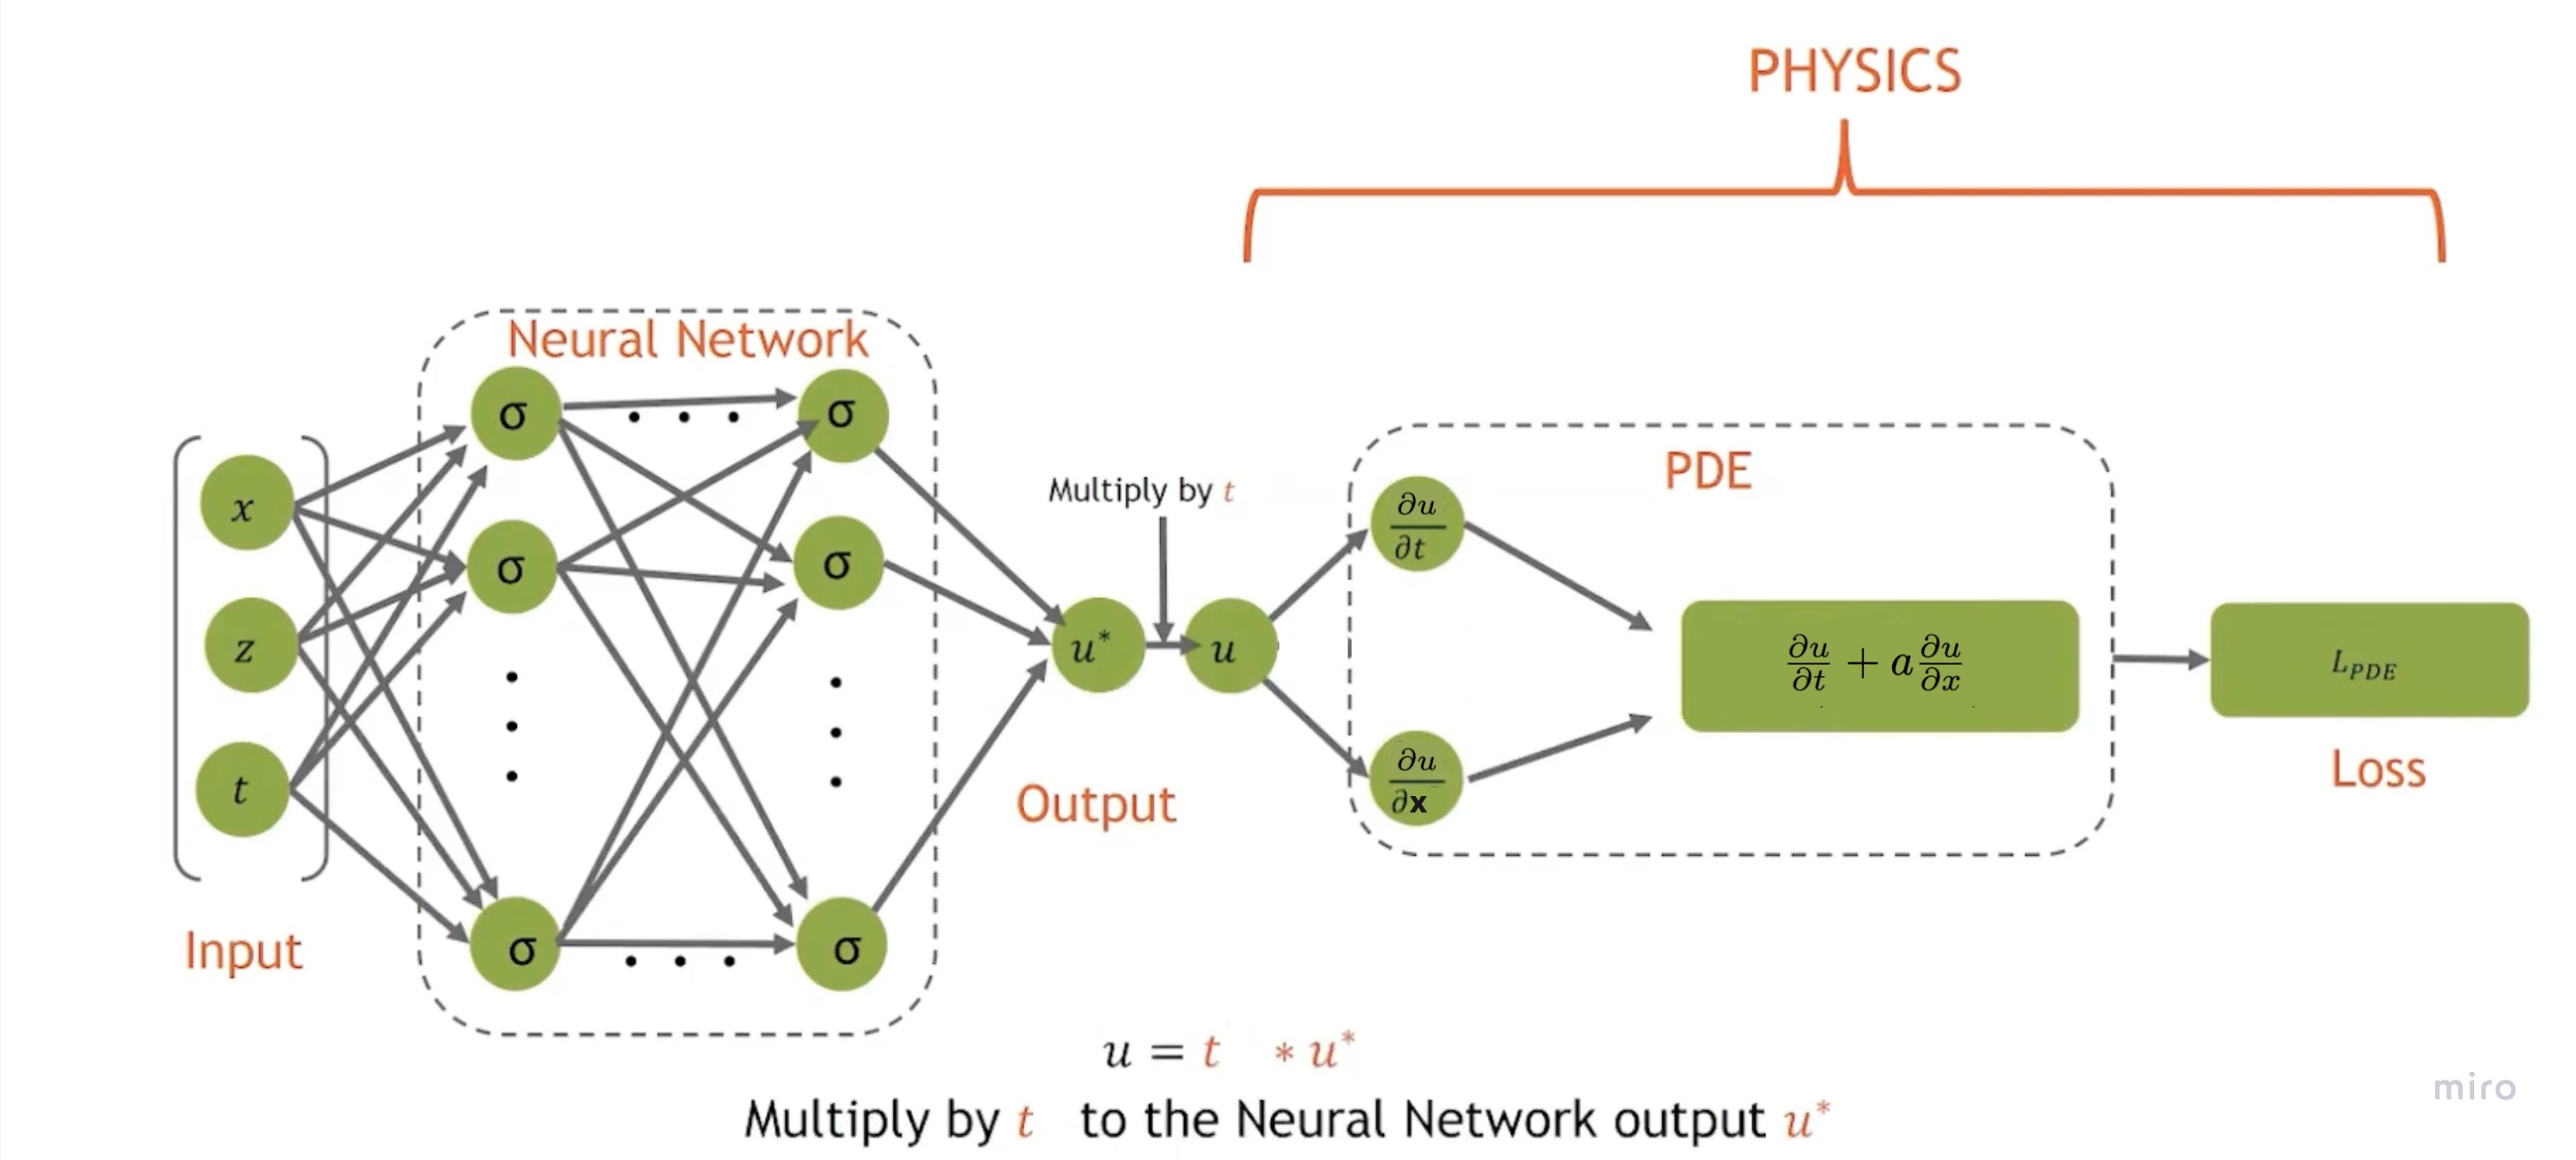
\includegraphics[width=0.9\textwidth]{images/loss.jpg}
    \caption{PINNs}
\end{figure}

\subsubsection{Convergence analysis}
One of the goals for the implementation of the PINN theory is to investigate the convergence and stability of the computed $u_\theta$ to the exact solution of the problem. They are related to how well the NN learns from physical laws and data.

%PENDIENTEEEEEE
% \subsubsection{Error analysis}
% We will be using the Mean Square Error (MSE) to measure the error of our neural network, we will be using the following formula:

% \begin{equation*}
%     MSE_{u_{exact}}=\frac{1}{N_{u_{exact}}}\sum^{N_{u_{exact}}}_{i=1}|u(t_{u_{exact}}^i,x_{u_{exact}}^i)-\overline{u_\theta}(t_{u_{exact}}^i,x_{u_{exact}}^i)|^2
% \end{equation*}

\section{Implementation}
Our main objective is to implement a solver that based on the Semi-Lagrangian scheme, and implementing the Deep Lagrange interpolation operator 
using the $u_\theta$ function that will be approximated by a neural network that implements the PINNs strategy will solve the equation (1) for different initial conditions depending on the values of $\mu$ and $\sigma$ for the Gaussian distribution and $A$ for the rectangular function.

\subsection{PINNs code}

We implement a Python code to approximate  $u_\theta$ that in our case is equal to the solution of the PDE, by using the PINNs strategy, for this we will be using the library PyTorch for machine learning.
The aim is to achieve a trained Neural Network that can give the output $u\theta(x, t)$, where x and t are set as inputs that satisfy Eq. (1). 

This PDE has an analytical exact solution which is $u(x,t) = u_0(x,x-at)$, where $u_0$ is the initial condition.

The fundamental concept is that by performing a forward pass through the network using the independent variables as inputs, we can obtain the corresponding evaluated dependent variables.
Since PINNs are derivable, we can compute the dependent variables (outputs). The dependent variables (inputs) to calculate the different derivatives that appear in the original PDEs. We create a loss function that fits the PDEs with this derivative throughout the training phase. 
We will assume that our PINNs solve the PDEs if the loss function approaches a near-zero value, the training can be done in both an unsupervised and supervised setting.\\

%NO ES UN BUEN LUGAR ACOMODAR
% We define the collocation and the data points, each of which would have a separate loss function that will be added together to form the total loss function.

% When $t = 0$, the initial condition will use a Mean Square Error (MSE) loss function, which will equate the known initial condition with the PINNs output. For the spatial boundary condition, 
% we use a periodic condition that compares the solutions using an MSE loss functionat $x=xmin$ and $x=xmax$ for any t and forces them to be equal. the same is done for the temporal boundary condition. 
% We characterize our solution as a NN with two inputs (number of independent variables), hidden layers, and one output that is defined as $\overline{u_\theta}(x,t)$, which is the approximation of the solution of the PDE given by the NN. 

%There are two approcahes to solve the PDEs using PINNs, the first one is Data-Driven and the othe rone is model based 
%Explicar por encima cada function y solo poner las mas importantes
%Description of the code implementation with some code snippets and explanations of the most important parts of the code.

\subsubsection{Neural Network Class}

The Net class represents a neural network model. It inherits from nn.DataParallel, which is a PyTorch module used for parallelizing the computation on multiple GPUs.
Our neural network contains 6 fully connected layers, an input layer that expects four or three input features x, t, mean, and variance/ A according to the initial condition, and five hidden layers, each consisting of fully connected linear units (nn.Linear) followed by the hyperbolic tangent activation function (torch.tanh). The hidden layers progressively reduce the input dimensions and extract higher-level features from the input data, 
and finally the output layer that consists of a single fully connected linear unit (nn.Linear) without an activation function. It maps the output of hidden layer5 to a single output value.

\subsubsection*{The forward method} Defines the forward pass of the neural network, where the input tensors propagate through the layers in a sequential manner, applying the specified operations and activation functions. The resulting output is returned as the final output of the network.

\subsubsection*{The networkBC method} Serves to impose the hard boundary condition, so when $t=0$ we get that the solution at that time is equal to the initial solution. 

\subsubsection{Parameters class} This class defines the set of parameters for the PINN class including the initial condition $u_0$ defined as a Gaussian distribution or a rectangular function.
\subsubsection{Network class} The Network class represents a \textbf{PINN} model.
\begin{enumerate}
    \item \textbf{\_\_init\_\_(param: Parameters)}: Initializes the neural network model and loads the model if available.

    \item \textbf{\_\_call\_\_(*args)}: Calls the network and returns the output.
    
    \item \textbf{create\_network()}: Creates the neural network model from the prevously defined Net class.
    
    \item \textbf{load(file\_name)}: Loads the model from a file. 
    
    \item \textbf{save(file\_name, epoch, net\_state, optimizer\_state, loss, loss\_history)}: Saves the model with the specific values passed as arguments into a file.
    
    \item \textbf{pde(x, t, mean, variance)}: Computes the PDE using the network and returns the result.
    
    \item \textbf{predict\_u\_from\_torch(x, t, mean, variance)}: Predicts the value of the solution given by the neural network based on the input variables $x$, $t$, \texttt{mean}, and \texttt{variance} or $A$
    
    \item \textbf{random(min\_value, max\_value, shape, requires\_grad=False, device=device)}: Generates random numbers within a range.
    
    \item \textbf{make\_data(n\_data)}: Generates the data of size \texttt{n\_data} for the training process based on the exact solution of the PDE.
    
    \item \textbf{make\_collocation(n\_collocation)}: Generates \texttt{n\_collocation} collocation points to enforce PDE constraints during training.
    
    \item \textbf{train(epochs, n\_collocation, n\_data)}: Trains the neural network using a combination of PDE constraints and data fitting.
    
    \item \textbf{u\_exact(x, t, a, xmax, u0, mean, variance, device=device)}: Computes the exact solution for the PDE.
    
    \item \textbf{plot(t, mean, variance)}: Plots the loss history, predicted solution, and prediction error at the input variables $x$, $t$, \texttt{mean}, and \texttt{variance}.

\end{enumerate}

\subsubsection{Optimization step}

The \textbf{train} function implements an optimization method for training a neural network by combining PDE constraints and data fitting. It iterates over a number of epochs to update the network's weights and minimize the loss.

% Within each epoch, the optimizer's gradients are reset to zero. The overall loss is set to zero to accumulate the losses from different components.

If there are collocation points specified, PDE constraints are enforced, collocation points are generated, and the network's output for these points is computed. Then the MSE loss is calculated between the network's output and a tensor of zeros, and this loss is added to the overall loss.

Similarly, if there are training data points specified, data fitting is performed, the raining data is generated, and then using the NN's prediction of the solution based on the input variables, then the MSE loss is computed between the predicted solution and the exact solution, and this loss is added to the overall loss.

Additional loss terms are incorporated to enforce PDE constraints and boundary conditions. The network's solution is evaluated at the boundary points and compared to the boundary values to enforce periodicity in both spatial and temporal dimensions, then the loss is added to the overall loss.

Backpropagation is then performed to compute the gradients, and the weights of the neural network are updated using the gradient descent algorithm.

Throughout the training process, the current loss is recorded in the loss history and the model and optimizer states, as well as the loss history, are saved for further analysis. Upon completion of all epochs, the best model is saved.

\subsection{Semi-Lagrangian solver}

We define a class called \textbf{SemiLagrangianSolver} that contains the following methods:

\begin{enumerate}
   \item \textbf{$u_0$}: To compute the initial condition.
   \item \textbf{explicit solution}: To compute the analytical solution
   \item \textbf{find closest}: To find the $n_{closests}$ points to $x_{*}$
   \item \textbf{li}: To compute the Lagrange interpolation basis polynomial at $x_{*}$
   \item \textbf{solver}: To calculate the numerical solution for the problem using the Lagrange interpolation operator.
   \item \textbf{plot solution}: To plot the solution at a specific time
   \item \textbf{error solution}: To calculate the error of the numerical solution compared to the exact solution
   \item \textbf{u theta}  The $u_{\Theta}$ solution found by the neural network.
   \item \textbf{solver deep} to calculate the solution of the transport equation using the Deep Lagrange Interpolation and $u_{\Theta}$.
   \item \textbf{plot solution deep} to plot the solution deep at a specific time
   \item \textbf{error solution deep} to calculate the error of the numerical deep solution compared to the exact solution
\end{enumerate}

And the following parameters: 

\begin{itemize}
    \item[--] $nx$ the number of points in the space
    \item[--] $nt$ the number of points in the time
    \item[--] $a$ the velocity of the transport
    \item[--] $\Delta t$ the time step
    \item[--] $\Delta x$ the space step
    \item[--] $t_{min}$ the minimum time
    \item[--] $t_{max}$ the maximum time
    \item[--] $x_{min}$ the minimum space
    \item[--] $x_{max}$ the maximum space
    \item[--] $u_0$ the initial condition
    \item[--] $u$ the solution
 \end{itemize}

\section{Results}

Here we present the results of the PINNs implementation, we will show the results of the unsupervised and supervised learning, we will also show the results of the deep interpolation method.

\subsection{Finding $u_\theta$ using PINNs}

In the following figures we show the results of the PINNs implementation, we will show the results of the unsupervised and supervised learning.\\

The training was done using the following parameters:

\begin{itemize}
   \item[--] epocs = 40000
   \item[--] ncollocation = 50000
   \item[--] ndata = 10000
\end{itemize} The best loss we obtained was: \textbf{7.80e-04} \\
For an initial solution with mean=0.5 and variance = 0.035 we get the following approximation made by the network at different time steps:\\

\begin{equation*}
    u_0(x) = \exp^{\frac{-(x-0.5)^2}{0.035}}
\end{equation*}

\begin{figure}[!h]
    \centering
    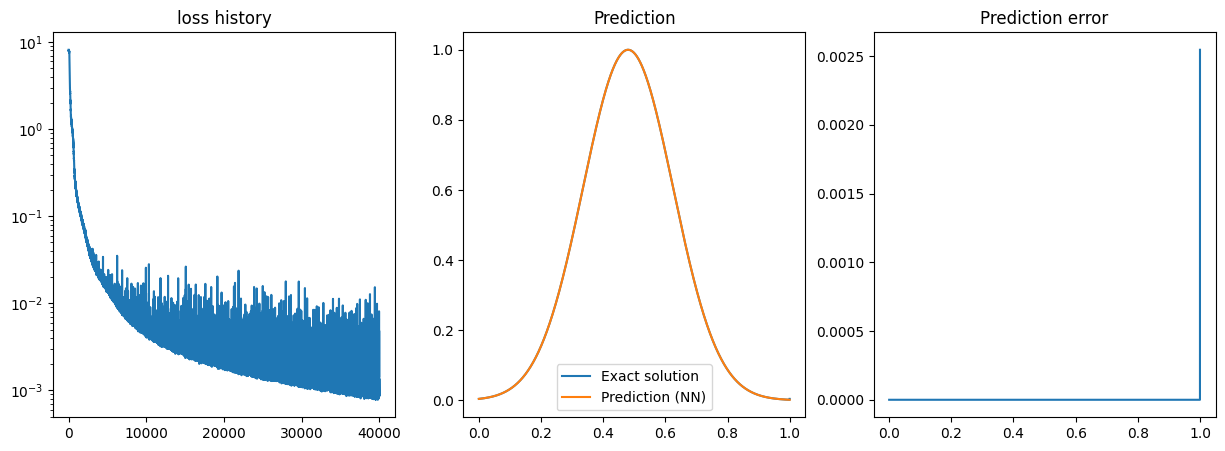
\includegraphics[width=0.5\textwidth]{images/r1.png}
    \caption{t=0}
% \end{figure}
% \begin{figure}[!h]
    % \centering
    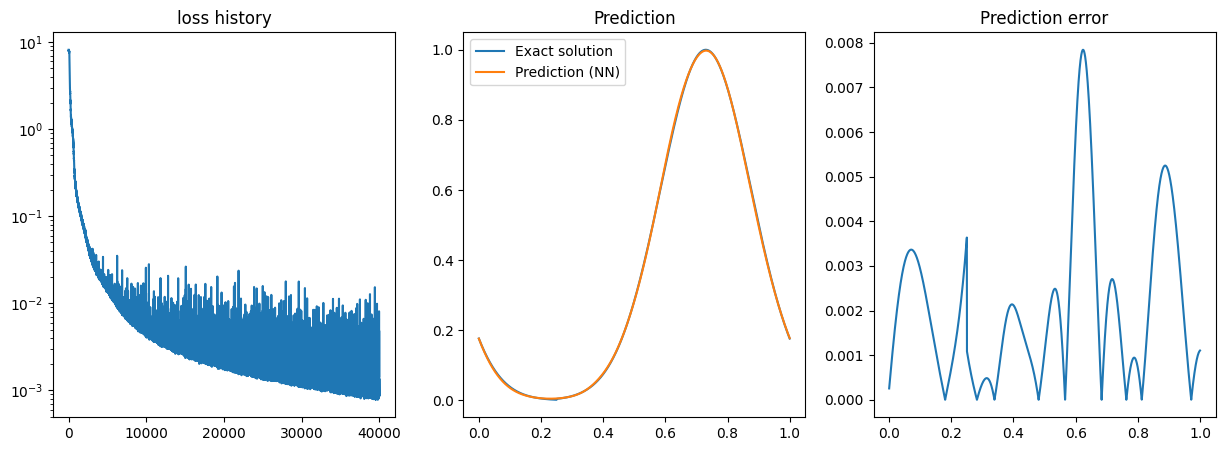
\includegraphics[width=0.5\textwidth]{images/r2.png}
    \caption{t=0.25}
% \end{figure}
% \begin{figure}[!h]
%     \centering
    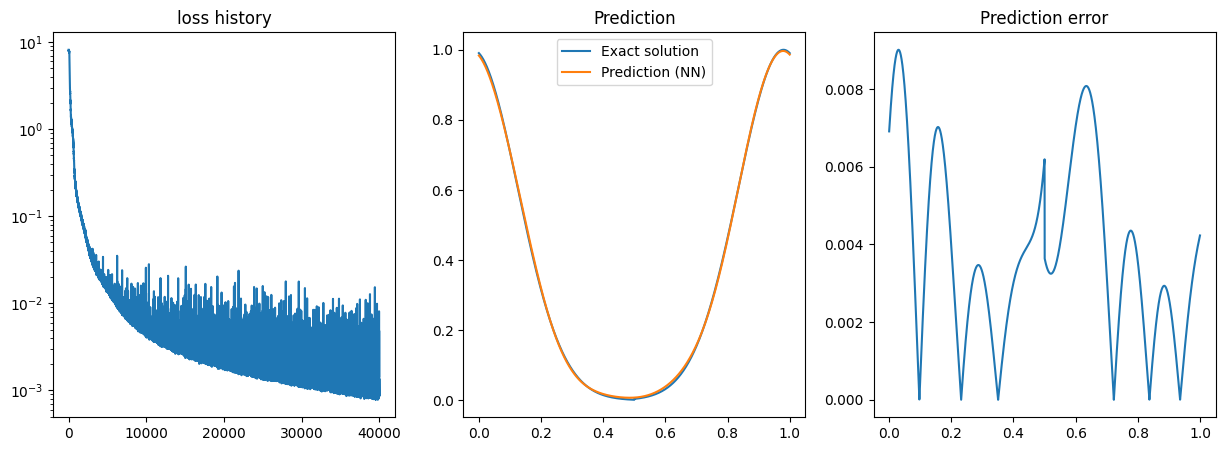
\includegraphics[width=0.5\textwidth]{images/r3.png}
    \caption{t=0.5}
% \end{figure}
% \begin{figure}[!h]
%     \centering
    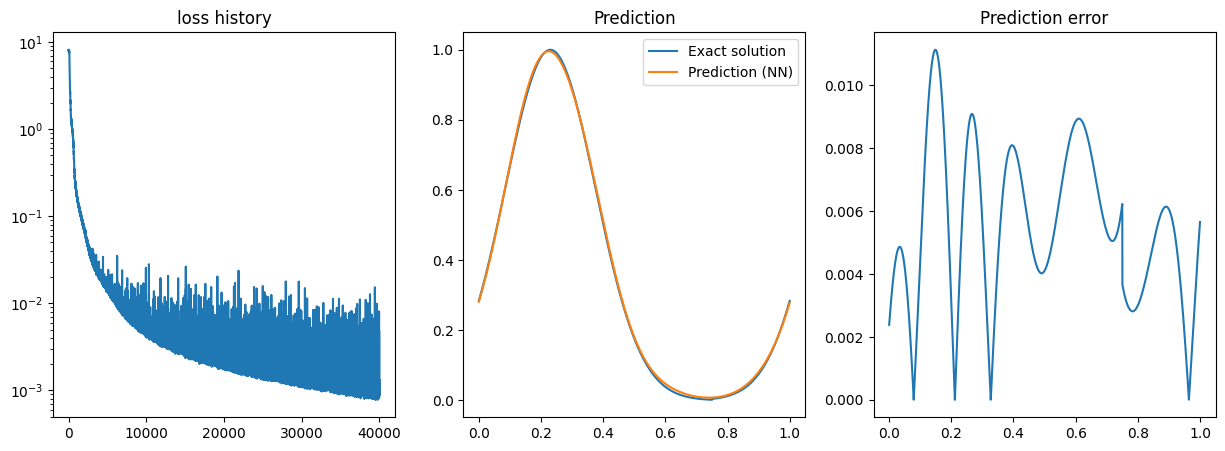
\includegraphics[width=0.5\textwidth]{images/r4.png}
    \caption{t=0.75}
% \end{figure}
% \begin{figure}[!h]
%     \centering
    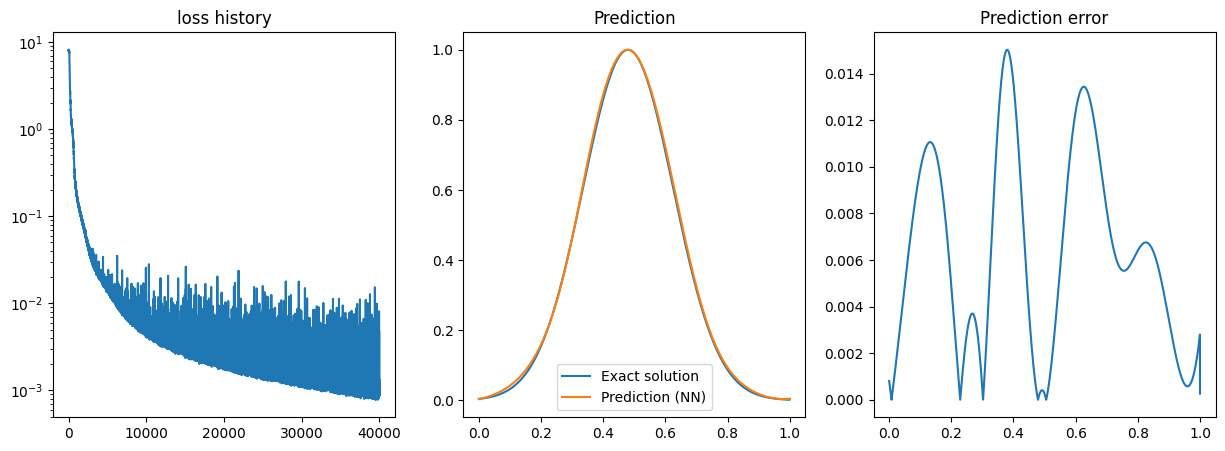
\includegraphics[width=0.5\textwidth]{images/r5.png}
    \caption{t=1}
\end{figure} 

For an initial solution defined by the following rectangular function:

\begin{equation*}
    u_0(x) = \begin{cases}
    0.6 & \text{if } 0.25 \leq x \leq 0.75\\
    0.3 & \text{otherwise}
    \end{cases}
\end{equation*} We obtained the following predictions:

\subsection{Solving using deep interpolation}
The following results were obtained using the following parameters:

\begin{itemize}
    \item[--]$xmin = 0.0$
    \item[--] $xmax = 1.0$
    \item[--] $tmin = 0.0$
    \item[--] $tf = 1.0$
    \item[--] $nt = 100$
    \item[--] $a = 1$
    \item[--] $mean = 0.5$
    \item[--] $variance = 0.035$
\end{itemize}

We obtained the following errors calculated in L2 norm compared to the exact solution (in loglog scale) of the transport equation according to the initial condition defined by the Gaussian with the mean and the variance given in parameter at times tf/4 tf /2 and tf (with tf the final time)
\subsection{Interpolation of order 1}

The \textbf{SL classic} solution is obtained with the Semi-Lagrangian scheme and the classic Lagrange interpolation, \textbf{SL Deep} is calculated using this time the deep interpolation operator and $u_\theta $ as the solution given by the neural network, \textbf{Network} is the solution obtained by the network.\\

\begin{figure}[!h]
    \centering
    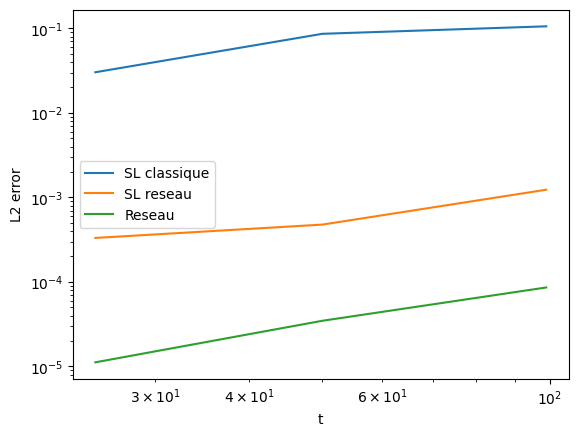
\includegraphics[width=0.4\textwidth]{images/i110.png}
    \caption{nx = 10}
    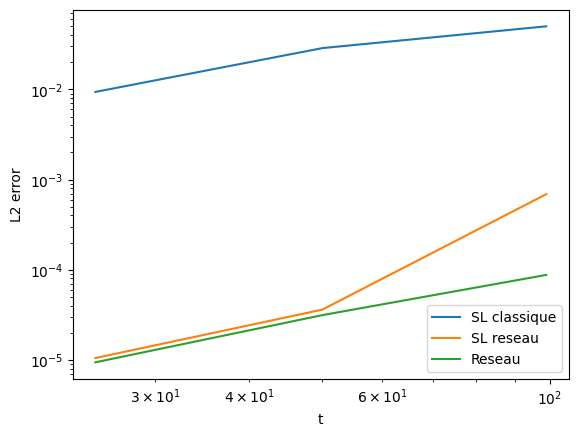
\includegraphics[width=0.4\textwidth]{images/i120.png}
    \caption{nx = 20}
    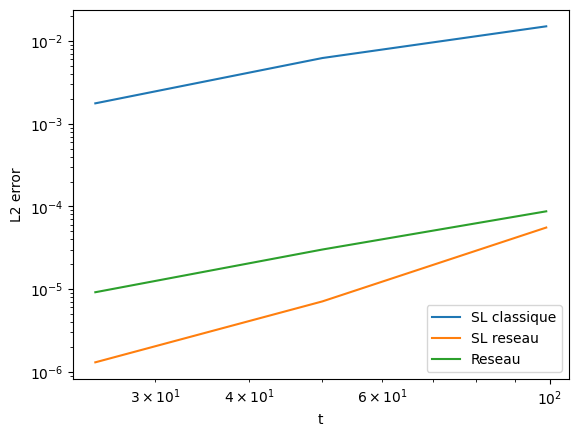
\includegraphics[width=0.4\textwidth]{images/i1.png}
    \caption{nx = 40}
\end{figure}

\newpage

The solution \textbf{perturbed SL} is defined as the exact solution to which we add different perturbations $\epsilon + \cos(x)$, here is what we get:\\

\begin{figure}[!h]
    \centering
    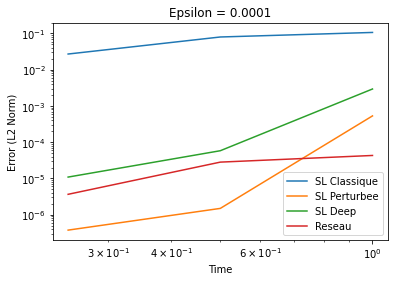
\includegraphics[width=0.45\textwidth]{images/10ep11.png}
    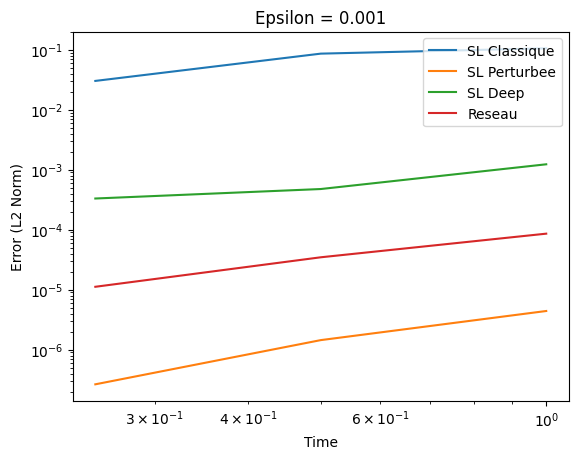
\includegraphics[width=0.45\textwidth]{images/10ep12.png}
    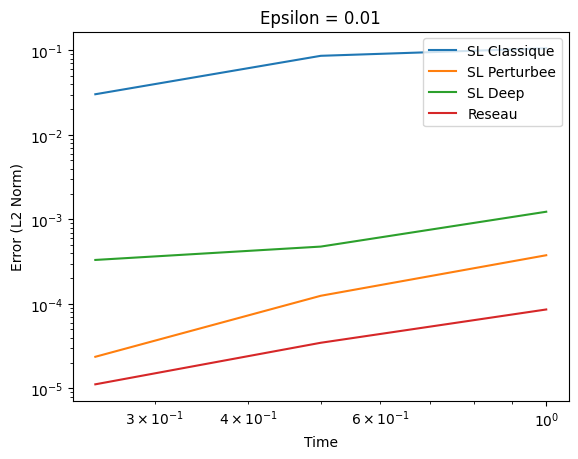
\includegraphics[width=0.45\textwidth]{images/10ep13.png}
    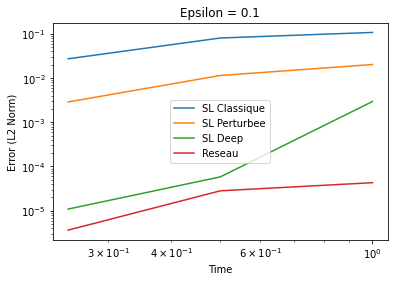
\includegraphics[width=0.45\textwidth]{images/10ep14.png}
    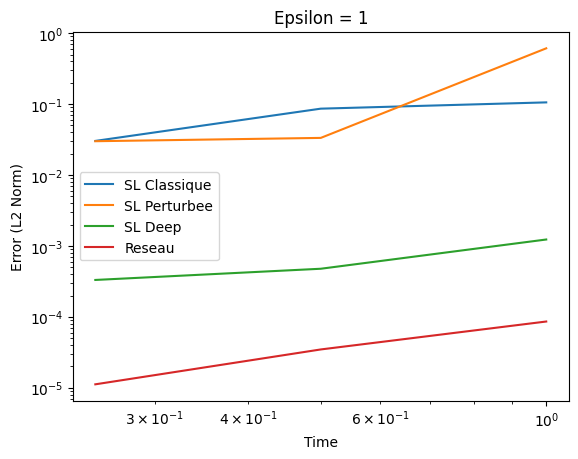
\includegraphics[width=0.45\textwidth]{images/10ep15.png}
    \caption{$nx = 10$}
\end{figure}

\newpage

\begin{figure}[!h]
    \centering
    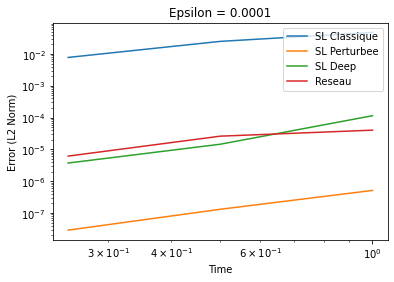
\includegraphics[width=0.45\textwidth]{images/20ep11.png}
    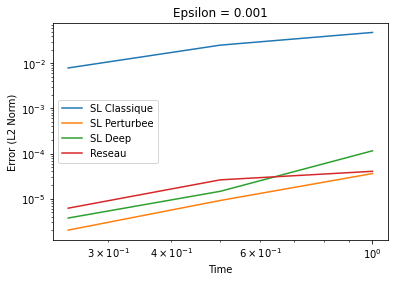
\includegraphics[width=0.45\textwidth]{images/20ep12.png}
    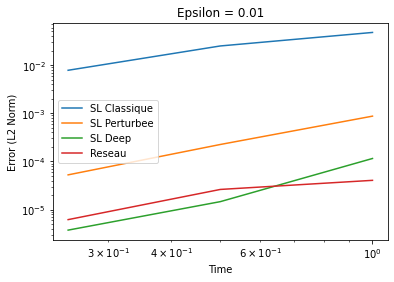
\includegraphics[width=0.45\textwidth]{images/20ep13.png}
    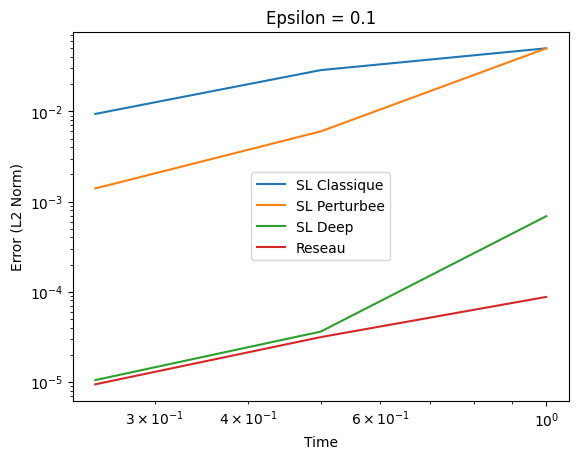
\includegraphics[width=0.45\textwidth]{images/20ep14.png}
    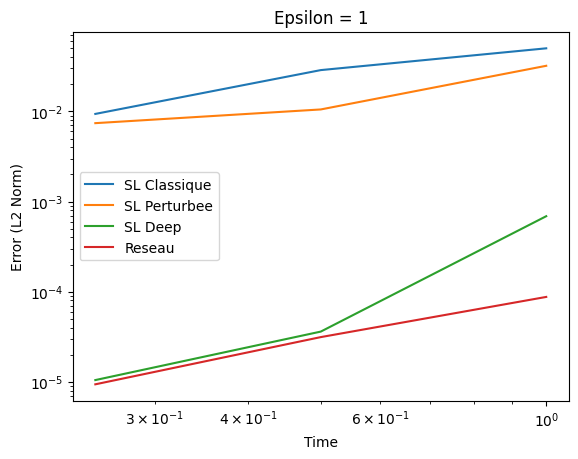
\includegraphics[width=0.45\textwidth]{images/20ep15.png}
    \caption{$nx = 20$}
\end{figure}

\newpage

\begin{figure}[!h]
    \centering
    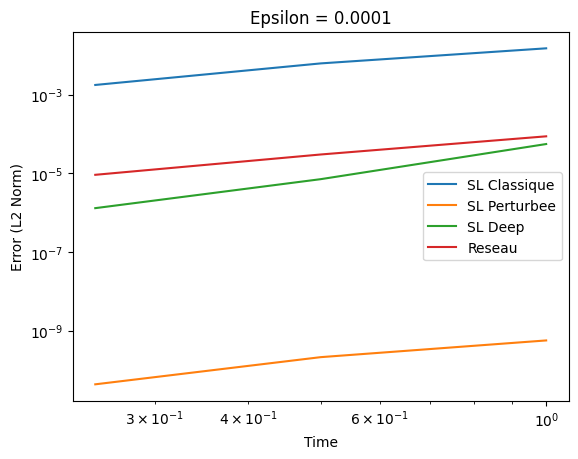
\includegraphics[width=0.45\textwidth]{images/ep11.png}
    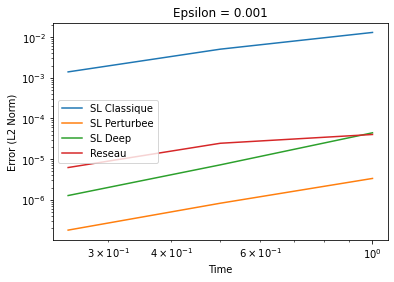
\includegraphics[width=0.45\textwidth]{images/ep12.png}
    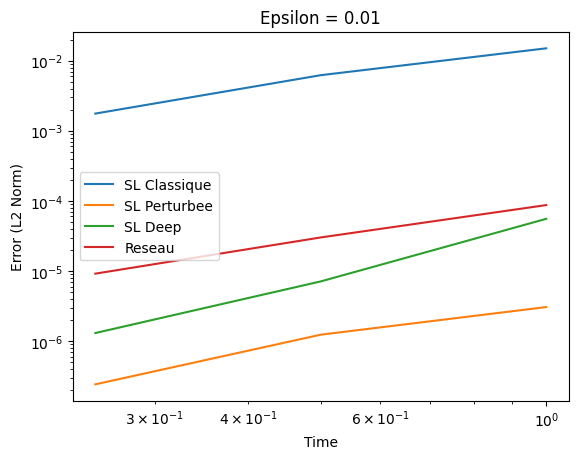
\includegraphics[width=0.45\textwidth]{images/ep13.png}
    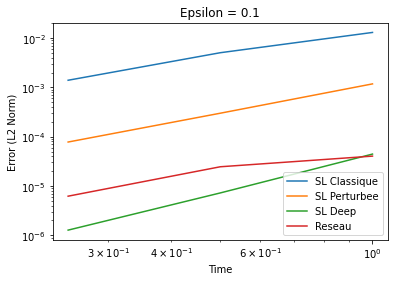
\includegraphics[width=0.45\textwidth]{images/ep14.png}
    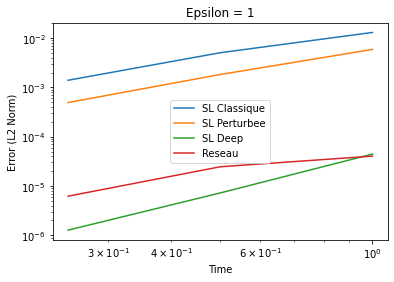
\includegraphics[width=0.45\textwidth]{images/ep15.png}
    \caption{$nx = 40$}
\end{figure}

\newpage 

\subsection{Interpolation of order 3}

The \textbf{SL classic} solution is obtained with the Semi-Lagrangian scheme and the classic Lagrange interpolation, \textbf{SL Deep} is calculated using this time the deep interpolation operator and $u_\theta $ as the solution given by the neural network, \textbf{Network} is the solution obtained by the network.\\

\begin{figure}[!h]
    \centering
    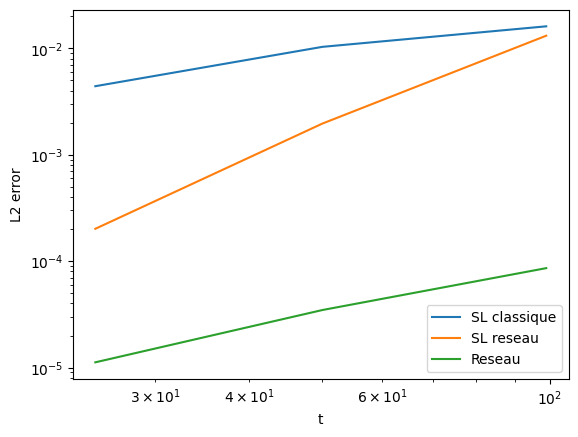
\includegraphics[width=0.5\textwidth]{images/i310.png}
    \caption{$nx = 10$}
    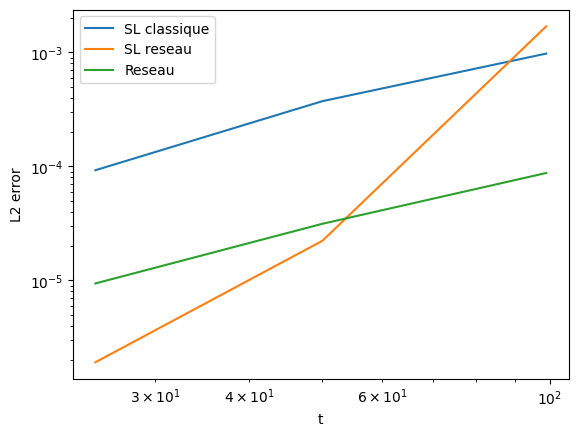
\includegraphics[width=0.5\textwidth]{images/i320.png}
    \caption{$nx = 20$}
    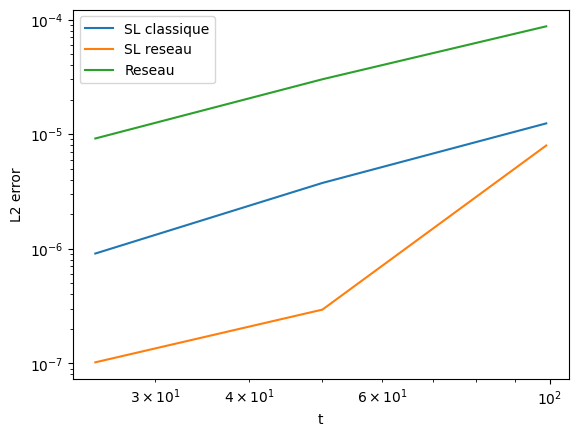
\includegraphics[width=0.5\textwidth]{images/i3.png}
    \caption{$nx = 40$}
\end{figure}

\vspace{4cm}

The solution \textbf{perturbed SL} is defined as the exact solution to which we add different perturbations $\epsilon + \cos(x)$, here is what we get:\\

\begin{figure}[!h]
    \centering
    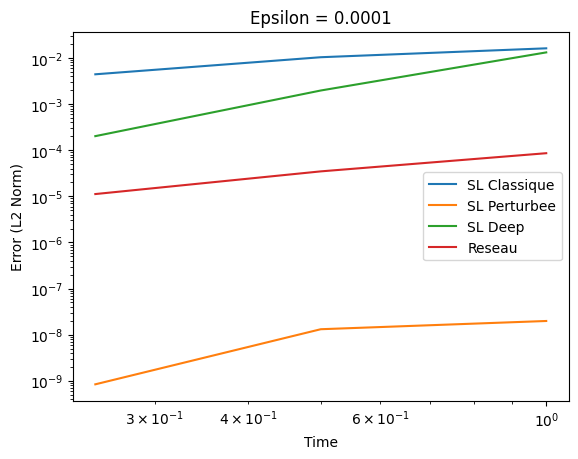
\includegraphics[width=0.49\textwidth]{images/10ep21.png}
    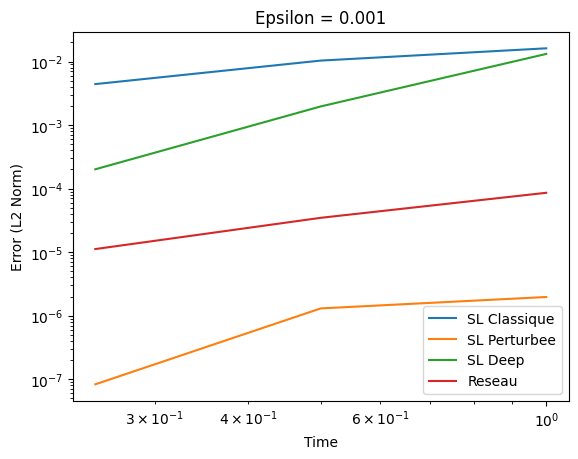
\includegraphics[width=0.49\textwidth]{images/10ep22.png}
    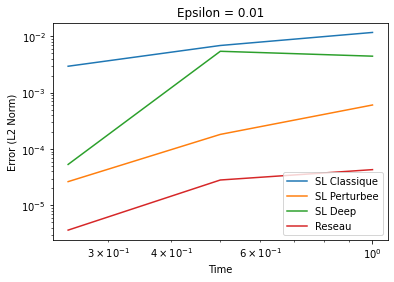
\includegraphics[width=0.49\textwidth]{images/10ep23.png}
    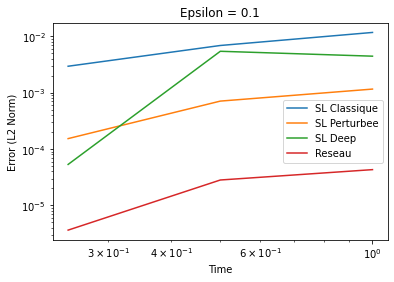
\includegraphics[width=0.49\textwidth]{images/10ep24.png}
    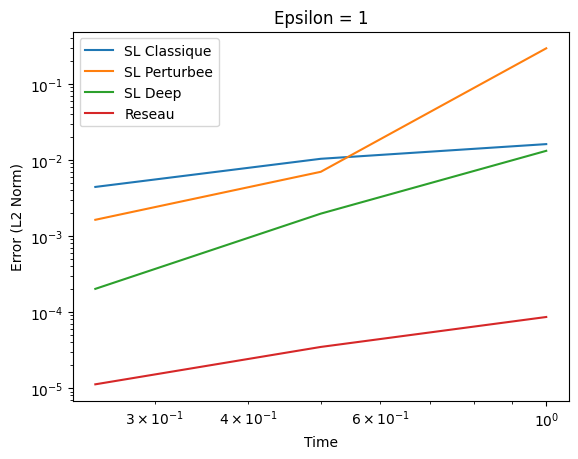
\includegraphics[width=0.49\textwidth]{images/10ep25.png}
    \caption{$nx = 10$}
\end{figure}

\newpage 

\begin{figure}[htbp]
    \centering
    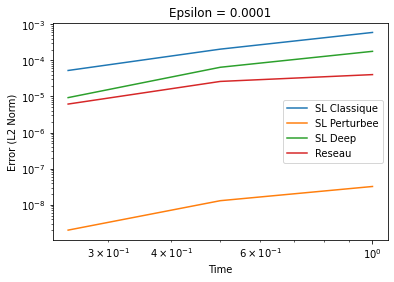
\includegraphics[width=0.49\textwidth]{images/20ep21.png}
    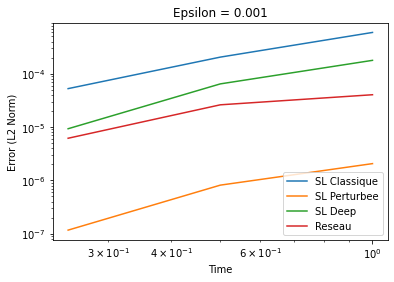
\includegraphics[width=0.49\textwidth]{images/20ep22.png}
    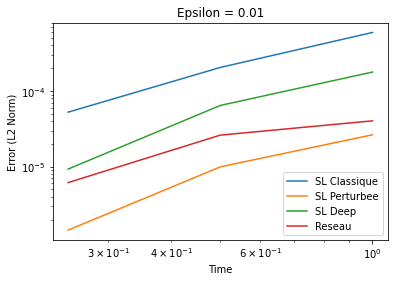
\includegraphics[width=0.49\textwidth]{images/20ep23.png}
    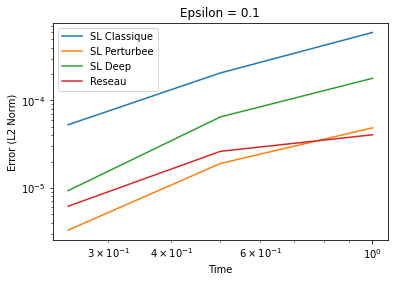
\includegraphics[width=0.49\textwidth]{images/20ep24.png}
    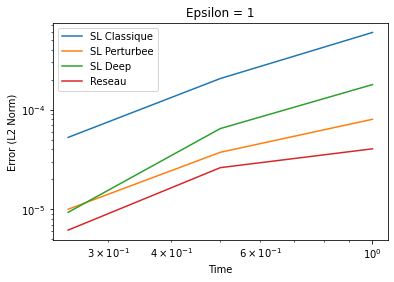
\includegraphics[width=0.49\textwidth]{images/20ep25.png}
    \caption{$nx = 20$}
\end{figure}

\begin{figure}[!h]
    \centering
    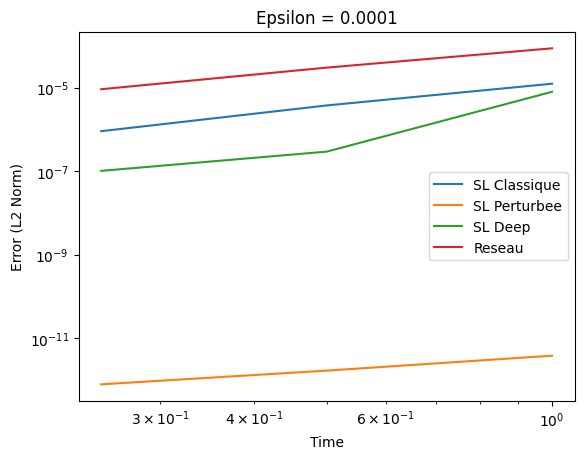
\includegraphics[width=0.48\textwidth]{images/ep21.png}
    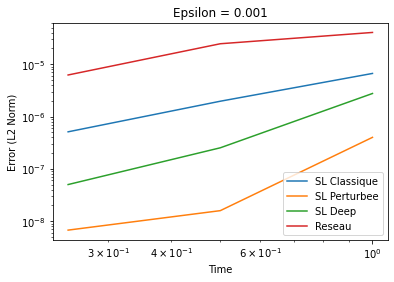
\includegraphics[width=0.48\textwidth]{images/ep22.png}
    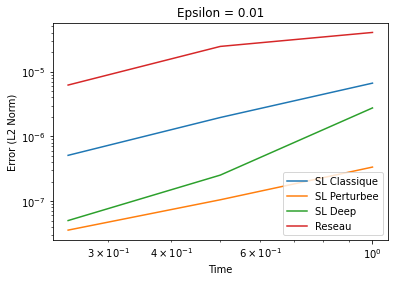
\includegraphics[width=0.48\textwidth]{images/ep23.png}
    \includegraphics[width=0.48\textwidth]{images/ep24.png}
    \includegraphics[width=0.48\textwidth]{images/ep25.png}
    \caption{$nx = 40$}
\end{figure}


\newlength{\customspace}
\setlength{\customspace}{2em}
\hspace{\customspace} 
\newpage

\subsection{Average gain}

By randomly drawing 20 parameters for the mean and the variance to have different initial conditions, we calculate for each the solution with the classic and deep Semi-Lagrangian method and we look at the gain=SL error/deep SL error by doing the average over the 20 parameters.\newline 

By making several draws of 20 parameters, the following average gains are obtained:

- For a 1st order interpolation: 137.7119541688143, 97.15674818809492, 185.7843283662372

- For an interpolation of order 3: 7.608668520339034, 3.1395029764283313,4.496461973620286

Then we can see that the gain is considerable when we use the deep interpolation operator, it is much less when we use the classic interpolation operator.\\



\section{Conclusions}


\section{Bibliography}
% \bibitem[label]{1} {Scientific Machine Learning Through Physics–Informed Neural Networks: Where we are and What’s Next}
% Salvatore Cuomo1 · Vincenzo Schiano Di Cola2 · Fabio Giampaolo1 · Gianluigi Rozza3 · Maziar Raissi4 · Francesco Piccialli1
% 26 July 2022
% \bibitem[label]{2} {Supervised vs. Unsupervised Learning: What’s the Difference?} {https://www.ibm.com/cloud/blog/supervised-vs-unsupervised-learning}
% \bibiitem[label]{3} {What are neural networks?} {https://www.ibm.com/topics/neural-networks}

% \bibiitem[label]{4} {Feed Forward Neural Network} {https://deepai.org/machine-learning-glossary-and-terms/feed-forward-neural-network}
% \bibiitem[label]{5} {What is a feedforward neural network?} {https://www.ibm.com/cloud/learn/feedforward-neural-network}
% \bibiitem[label]{6} {Multilayer Perceptron Explained with a Real-Life Example and Python Code} {https://towardsdatascience.com/multilayer-perceptron-explained-with-a-real-life-example-and-python-code-sentiment-analysis-cb408ee93141}
% \bibiitem[label]{7} {https://www.pnas.org/doi/full/10.1073/pnas.1718942115}
\end{document}

